\begin{frame}
	\myheading{Module 18.2: Factors in Markov Network}
\end{frame}

\begin{frame}
	\begin{columns}
		\column{0.5\textwidth}
		\begin{overlayarea}{\textwidth}{\textheight}
		\vspace{0.1in}
		\begin{center}
                \tikzstyle{input_neuron}=[ellipse,draw=red!50,fill=orange!10,thick,scale=0.7]
                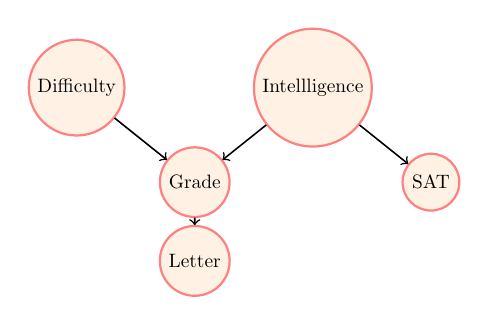
\begin{tikzpicture}
                    \node [input_neuron](input0) at (7,-0.1)  {Grade};
                    \node [input_neuron] (input1) at (10,-0.1)  {SAT};
                    \node [input_neuron] (input2) at (8.5, 1.1) {Intellligence};
                    \node [input_neuron] (input3) at (7, -1.1) {Letter};
                    \node [input_neuron](input4) at (5.5,1.1)  {Difficulty};

                    \draw [line width=0.2mm, ->] (input2) -- (input0);
                    \draw [line width=0.2mm, ->] (input0) -- (input3);
                    \draw [line width=0.2mm, ->] (input2) -- (input1);
                    \draw [line width=0.2mm, ->] (input4) -- (input0);
                \end{tikzpicture}
            \end{center}
         \vspace{0.1in}
        \begin{align*}
        P(G,&S,I,L,D) = \\
        &P(I)P(D)P(G|I,D)P(S|I)P(L|G)
        \end{align*}
		\end{overlayarea}
		\column{0.5\textwidth}
		\begin{overlayarea}{\textwidth}{\textheight}
			\begin{itemize}\justifying
			\item<1-> Recall that in the directed case the factors were Conditional Probability Distributions (CPDs)
			\item<2-> Each such factor captured interaction (dependence) between the connected nodes
			\item<3-> Can we use CPDs in the undirected case also ?
			\item<4-> CPDs don't make sense in the undirected case because there is no direction and hence no 
			natural conditioning (Is $A|B$ or $B|A$?)
			\end{itemize}
		\end{overlayarea}
	\end{columns}
\end{frame}

\begin{frame}
	\begin{columns}
		\column{0.5\textwidth}
		\begin{overlayarea}{\textwidth}{\textheight}
		\vspace{0.1in}
		\begin{center}
				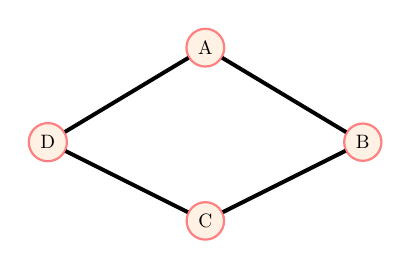
\begin{tikzpicture}
				\node [input_neuron](input0) at (5.5,-0.1)  {D};
				\node [input_neuron] (input1) at (9.5,-0.1)  {B};
				\node [input_neuron] (input2) at (7.5, 1.1) {A};
				\node [input_neuron] (input3) at (7.5, -1.1) {C};

				\draw [line width=0.5mm, -] (input2) -- (input0);
				\draw [line width=0.5mm, -] (input2) -- (input1);
				\draw [line width=0.5mm, -] (input0) -- (input3);
				\draw [line width=0.5mm, -] (input1) -- (input3);
		\end{tikzpicture}
		\end{center}
		\end{overlayarea}
		\column{0.5\textwidth}
		\begin{overlayarea}{\textwidth}{\textheight}
			\begin{itemize}\justifying
			\item<1-> So what should be the factors or parameters in this case
			\item<2-> \textbf{Question:} What do we want these factors to capture ?
			\item<3-> \textbf{Answer:} The affinity between connected random variables
			\item<4-> Just as in the directed case the factors captured the conditional dependence between a set of random 
			variables, here we want them to capture the affinity between them
			\end{itemize}
		\end{overlayarea}
	\end{columns}
\end{frame}

\begin{frame}
	\begin{columns}
		\column{0.5\textwidth}
		\begin{overlayarea}{\textwidth}{\textheight}
		\vspace{0.1in}
		\begin{center}
				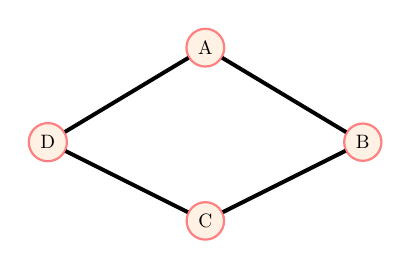
\begin{tikzpicture}
				\node [input_neuron](input0) at (5.5,-0.1)  {D};
				\node [input_neuron] (input1) at (9.5,-0.1)  {B};
				\node [input_neuron] (input2) at (7.5, 1.1) {A};
				\node [input_neuron] (input3) at (7.5, -1.1) {C};

				\draw [line width=0.5mm, -] (input2) -- (input0);
				\draw [line width=0.5mm, -] (input2) -- (input1);
				\draw [line width=0.5mm, -] (input0) -- (input3);
				\draw [line width=0.5mm, -] (input1) -- (input3);
		\end{tikzpicture}
		\end{center}
		\end{overlayarea}
		\column{0.5\textwidth}
		\begin{overlayarea}{\textwidth}{\textheight}
			\begin{itemize}\justifying
			\item<1-> However we can borrow the intuition from the directed case.
			\item<2-> Even in the undirected case, we want each such factor to capture interactions (affinity) between connected nodes
			\item<3-> We could have factors $\phi_1(A,B)$, $\phi_2(B,C)$, $\phi_3(C,D)$, $\phi_4(D,A)$ which capture the affinity between the corresponding nodes.
			\end{itemize}
		\end{overlayarea}
	\end{columns}
\end{frame}

\begin{frame}
	\begin{columns}
		\column{0.5\textwidth}
		\begin{overlayarea}{\textwidth}{\textheight}
		\vspace{0.1in}
		\begin{center}
				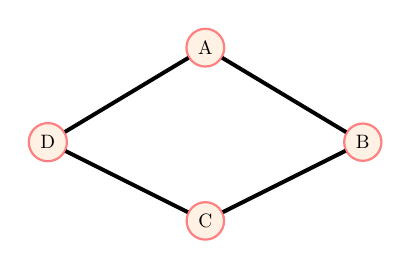
\begin{tikzpicture}
				\node [input_neuron](input0) at (5.5,-0.1)  {D};
				\node [input_neuron] (input1) at (9.5,-0.1)  {B};
				\node [input_neuron] (input2) at (7.5, 1.1) {A};
				\node [input_neuron] (input3) at (7.5, -1.1) {C};

				\draw [line width=0.5mm, -] (input2) -- (input0);
				\draw [line width=0.5mm, -] (input2) -- (input1);
				\draw [line width=0.5mm, -] (input0) -- (input3);
				\draw [line width=0.5mm, -] (input1) -- (input3);
		\end{tikzpicture}
		\end{center}
		\vspace{-0.2in}
		\begin{center}
		\begin{table}
\only<1>{\scalebox{0.6}{
\begin{tabular}{|ccp{1cm}|ccp{1cm}|ccp{1cm}|ccp{1cm}|}
\hline
\multicolumn{3}{|c|}{$\phi_1(A,B)$} & \multicolumn{3}{c|}{$\phi_2(B,C)$} & \multicolumn{3}{c|}{$\phi_3(C,D)$} & \multicolumn{3}{c|}{$\phi_4(D,A)$} \\ \hline
$a^0$        & $b^0$       &        & $a^0$        & $b^0$       &        & $a^0$       & $b^0$       &        & $a^0$       & $b^0$       &        \\
$a^0$        & $b^1$       &        & $a^0$        & $b^1$       &        & $a^0$       & $b^1$       &        & $a^0$       & $b^1$       &        \\
$a^1$        & $b^0$       &        & $a^1$        & $b^0$       &        & $a^1$       & $b^0$       &        & $a^1$       & $b^0$       &        \\
$a^1$        & $b^1$       &        & $a^1$        & $b^1$       &        & $a^1$       & $b^1$       &        & $a^1$       & $b^1$       &        \\ \hline
\end{tabular}}}
\only<2->{
	\scalebox{0.6}{
\begin{tabular}{|ccp{1cm}|ccp{1cm}|ccp{1cm}|ccp{1cm}|}
\hline
\multicolumn{3}{|c|}{$\phi_1(A,B)$} & \multicolumn{3}{c|}{$\phi_2(B,C)$} & \multicolumn{3}{c|}{$\phi_3(C,D)$} & \multicolumn{3}{c|}{$\phi_4(D,A)$} \\ \hline
$a^0$       & $b^0$       & 30      & $a^0$       & $b^0$      & 100      & $a^0$      & $b^0$      & 1        & $a^0$      & $b^0$      & 100      \\
$a^0$       & $b^1$       & 5       & $a^0$       & $b^1$      & 1        & $a^0$      & $b^0$      & 100      & $a^0$      & $b^1$      & 1        \\
$a^1$       & $b^0$       & 1       & $a^1$       & $b^0$      & 1        & $a^1$      & $b^1$      & 100      & $a^1$      & $b^0$      & 1        \\
$a^1$       & $b^1$       & 10      & $a^1$       & $b^1$      & 100      & $a^1$      & $b^1$      & 1        & $a^1$      & $b^1$      & 100      \\ \hline
\end{tabular}}
}
\end{table}
\end{center}
\vspace{-0.3in}
\footnotesize
\begin{itemize}\justifying
	\item<3-> But who will give us these values ?
	\item<4-> Well now you need to learn them from data (same as in the directed case)
	\item<5-> If you have access to a lot of past interactions between $A\&B$ then you could learn these values(more on this later)
	\end{itemize}
		\end{overlayarea}
		\column{0.5\textwidth}
		\begin{overlayarea}{\textwidth}{\textheight}

			\begin{itemize}\justifying
			\item<1-> Intuitively, it makes sense to have these factors associated with each pair of connected random variables.
			\item<2-> We could now assign some values of these factors
			\item<6-> Roughly speaking $\phi_1(A, B)$ asserts that it is more likely for $A$ and $B$ to agree [$\because$ weights for $a^0 b^0, a^1 b^1 > a^0b^1,a^1b^0]$
			\item <7-> $\phi_1(A,B)$ also assigns more weight to the case when both do not have a misconception as compared to the case when both have the misconception $a^0 b^0 > a^1b^1$
			\item<8-> We could have similar assignments for the other factors
			\end{itemize}
		\end{overlayarea}
	\end{columns}
\end{frame}


\begin{frame}
	\begin{columns}
		\column{0.5\textwidth}
		\begin{overlayarea}{\textwidth}{\textheight}
		\vspace{0.1in}
		\begin{center}
				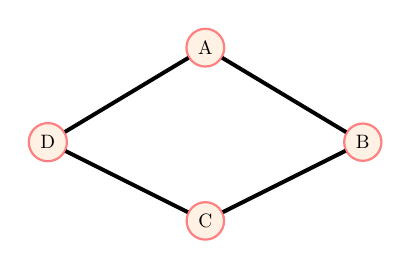
\begin{tikzpicture}
				\node [input_neuron](input0) at (5.5,-0.1)  {D};
				\node [input_neuron] (input1) at (9.5,-0.1)  {B};
				\node [input_neuron] (input2) at (7.5, 1.1) {A};
				\node [input_neuron] (input3) at (7.5, -1.1) {C};

				\draw [line width=0.5mm, -] (input2) -- (input0);
				\draw [line width=0.5mm, -] (input2) -- (input1);
				\draw [line width=0.5mm, -] (input0) -- (input3);
				\draw [line width=0.5mm, -] (input1) -- (input3);
		\end{tikzpicture}
		\vspace{-0.2in}
		\begin{table}
\scalebox{0.6}{
\begin{tabular}{|ccp{1cm}|ccp{1cm}|ccp{1cm}|ccp{1cm}|}
\hline
\multicolumn{3}{|c|}{$\phi_1(A,B)$} & \multicolumn{3}{c|}{$\phi_2(B,C)$} & \multicolumn{3}{c|}{$\phi_3(C,D)$} & \multicolumn{3}{c|}{$\phi_4(D,A)$} \\ \hline
$a^0$       & $b^0$       & 30      & $a^0$       & $b^0$      & 100      & $a^0$      & $b^0$      & 1        & $a^0$      & $b^0$      & 100      \\
$a^0$       & $b^1$       & 5       & $a^0$       & $b^1$      & 1        & $a^0$      & $b^0$      & 100      & $a^0$      & $b^1$      & 1        \\
$a^1$       & $b^0$       & 1       & $a^1$       & $b^0$      & 1        & $a^1$      & $b^1$      & 100      & $a^1$      & $b^0$      & 1        \\
$a^1$       & $a^1$       & 10      & $a^1$       & $b^1$      & 100      & $a^1$      & $b^1$      & 1        & $a^1$      & $b^1$      & 100      \\ \hline
\end{tabular}}
\end{table}
\end{center}
		\end{overlayarea}
		\column{0.5\textwidth}
		\begin{overlayarea}{\textwidth}{\textheight}
		\begin{itemize}\justifying
			\item<1-> Notice a few things
			\item<2-> These tables do not represent probability distributions
			\item<3-> They are just weights which can be interpreted as the relative likelihood of an event 
			\item<4-> For example, $a=0, b=0$ is more likely than $a=1, b=1$
		\end{itemize}
		\end{overlayarea}
	\end{columns}
	\end{frame}

\begin{frame}
	\begin{columns}
		\column{0.5\textwidth}
		\begin{overlayarea}{\textwidth}{\textheight}
		\vspace{0.1in}
		\begin{center}
				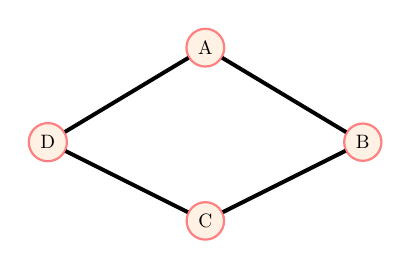
\begin{tikzpicture}
				\node [input_neuron](input0) at (5.5,-0.1)  {D};
				\node [input_neuron] (input1) at (9.5,-0.1)  {B};
				\node [input_neuron] (input2) at (7.5, 1.1) {A};
				\node [input_neuron] (input3) at (7.5, -1.1) {C};

				\draw [line width=0.5mm, -] (input2) -- (input0);
				\draw [line width=0.5mm, -] (input2) -- (input1);
				\draw [line width=0.5mm, -] (input0) -- (input3);
				\draw [line width=0.5mm, -] (input1) -- (input3);
		\end{tikzpicture}
		\vspace{-0.2in}
		\begin{table}
\scalebox{0.6}{
\begin{tabular}{|ccp{1cm}|ccp{1cm}|ccp{1cm}|ccp{1cm}|}
\hline
\multicolumn{3}{|c|}{$\phi_1(A,B)$} & \multicolumn{3}{c|}{$\phi_2(B,C)$} & \multicolumn{3}{c|}{$\phi_3(C,D)$} & \multicolumn{3}{c|}{$\phi_4(D,A)$} \\ \hline
$a^0$       & $b^0$       & 30      & $a^0$       & $b^0$      & 100      & $a^0$      & $b^0$      & 1        & $a^0$      & $b^0$      & 100      \\
$a^0$       & $b^1$       & 5       & $a^0$       & $b^1$      & 1        & $a^0$      & $b^0$      & 100      & $a^0$      & $b^1$      & 1        \\
$a^1$       & $b^0$       & 1       & $a^1$       & $b^0$      & 1        & $a^1$      & $b^1$      & 100      & $a^1$      & $b^0$      & 1        \\
$a^1$       & $a^1$       & 10      & $a^1$       & $b^1$      & 100      & $a^1$      & $b^1$      & 1        & $a^1$      & $b^1$      & 100      \\ \hline
\end{tabular}}
\end{table}
\end{center}
		\end{overlayarea}
		\column{0.5\textwidth}
		\begin{overlayarea}{\textwidth}{\textheight}
		\begin{itemize}\justifying
			\item<1-> But eventually we are interested in probability distributions
			\item<2-> In the directed case going from factors to a joint probability distribution was easy as the factors were themselves conditional probability distributions
			\item <3->We could just write the joint probability distribution as the product of the factors (without violating the axioms of probability)
			\item<4-> What do we do in this case when the factors are not probability distributions
		\end{itemize}
		\end{overlayarea}
	\end{columns}
	\end{frame}


\begin{frame}
	\begin{columns}
		\column{0.45\textwidth}
		\begin{overlayarea}{\textwidth}{\textheight}
		\begin{center}
		\begin{table}
		\scalebox{0.7}{
\begin{tabular}{|cccc|r|r|}
\hline
\multicolumn{4}{|c|}{\textit{\textbf{Assignment}}} & \multicolumn{1}{c|}{\textit{\textbf{Unnormalized}}} & \multicolumn{1}{c|}{\textit{\textbf{Normalized}}} \\ \hline
$a^0$       & $b^0$      & $c^0$      & $d^0$      & 300,000                                             & 4.17E-02                                          \\
$a^0$       & $b^0$      & $c^0$      & $d^1$      & 300,000                                             & 4.17E-02                                          \\
$a^0$       & $b^0$      & $c^1$      & $d^0$      & 300,000                                             & 4.17E-02                                          \\
$a^0$       & $b^0$      & $c^1$      & $d^1$      & 30                                                  & 4.17E-06                                          \\
$a^0$       & $b^1$      & $c^0$      & $d^0$      & 500                                                 & 6.94E-05                                          \\
$a^0$       & $b^1$      & $c^0$      & $d^1$      & 500                                                 & 6.94E-05                                          \\
$a^0$       & $b^1$      & $c^1$      & $d^0$      & 5,000,000                                           & 6.94E-01                                          \\
$a^0$       & $b^1$      & $c^1$      & $d^1$      & 500                                                 & 6.94E-05                                          \\
$a^1$       & $b^0$      & $c^0$      & $d^0$      & 100                                                 & 1.39E-05                                          \\
$a^1$       & $b^0$      & $c^0$      & $d^1$      & 1,000,000                                           & 1.39E-01                                          \\
$a^1$       & $b^0$      & $c^1$      & $d^0$      & 100                                                 & 1.39E-05                                          \\
$a^1$       & $b^0$      & $c^1$      & $d^1$      & 100                                                 & 1.39E-05                                          \\
$a^1$       & $b^1$      & $c^0$      & $d^0$      & 10                                                  & 1.39E-06                                          \\
$a^1$       & $b^1$      & $c^0$      & $d^1$      & 100,000                                             & 1.39E-02                                          \\
$a^1$       & $b^1$      & $c^1$      & $d^0$      & 100,000                                             & 1.39E-02                                          \\
$a^1$       & $b^1$      & $c^1$      & $d^1$      & 100,000                                             & 1.39E-02                                          \\ \hline
\end{tabular}}
		\end{table}
		\end{center}
		\end{overlayarea}
		\column{0.55\textwidth}
		\begin{overlayarea}{\textwidth}{\textheight}
		\begin{itemize}\justifying
			\item<1-> Well we could still write it as a product of these factors \onslide<+-> and normalize it appropriately
			\onslide<2->{
			\begin{align*}
			P(a,b,c,d) &= \\
			& \frac{1}{Z}{\phi_1(a,b)\phi_2(b,c)\phi_3(c,d)\phi_4(d,a)}
			\end{align*}}
			\onslide<3->{where 
			\begin{align*}
			Z = \sum_{a,b,c,d} \phi_1(a,b)\phi_2(b,c)\phi_3(c,d)\phi_4(d,a)
			\end{align*}}
			\item<4-> Based on the values that we had assigned to the factors we can now compute the full joint probability distribution
			\item<5-> $Z$ is called the partition function.
		\end{itemize}
		\end{overlayarea}
	\end{columns}
\end{frame}


\begin{frame}
	\begin{columns}
		\column{0.5\textwidth}
		\begin{overlayarea}{\textwidth}{\textheight}
			\vspace{1cm}
			\centering
			\onslide<2->{\tikzstyle{input_neuron}=[circle,draw=red!50,fill=orange!10,thick,scale=0.7]
			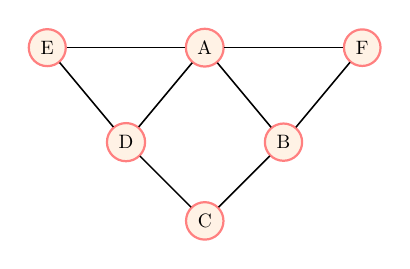
\begin{tikzpicture}
				\node [input_neuron](input0) at (6.5,-0.1)  {D};
				\node [input_neuron] (input1) at (8.5,-0.1)  {B};
				\node [input_neuron] (input2) at (7.5, 1.1) {A};
				\node [input_neuron] (input3) at (7.5, -1.1) {C};
				\node [input_neuron](input4) at (5.5,1.1)  {E};
				\node [input_neuron](input5) at (9.5,1.1)  {F};

				\draw [line width=0.2mm, -] (input0) -- (input2);
				\draw [line width=0.2mm, -] (input0) -- (input3);
				\draw [line width=0.2mm, -] (input1) -- (input2);
				\draw [line width=0.2mm, -] (input1) -- (input3);
				\draw [line width=0.2mm, -] (input0) -- (input4);
				\draw [line width=0.2mm, -] (input2) -- (input4);
				\draw [line width=0.2mm, -] (input1) -- (input5);
				\draw [line width=0.2mm, -] (input2) -- (input5);
			\end{tikzpicture}
			}
		\end{overlayarea}
		\column{0.5\textwidth}
		\begin{overlayarea}{\textwidth}{\textheight}
			\begin{itemize}\justifying
				\item<1-> Let us build on the original example by adding some more students
				\item<3-> Once again there is an edge between two students if they study together
				\item<4-> One way of interpreting these new connections is that $\{A,D,E\}$ from a study group or a clique
				\item<5-> Similarly $\{A,F,B\}$ form a study group and $\{C,D\}$ form a study group and $\{B,C\}$ form a study group
			\end{itemize}
		\end{overlayarea}
	\end{columns}
\end{frame}

\begin{frame}
	\begin{columns}
		\column{0.5\textwidth}
		\begin{overlayarea}{\textwidth}{\textheight}
			\vspace{1cm}
			\centering
			\onslide<1->{\tikzstyle{input_neuron}=[circle,draw=red!50,fill=orange!10,thick,scale=0.7]
			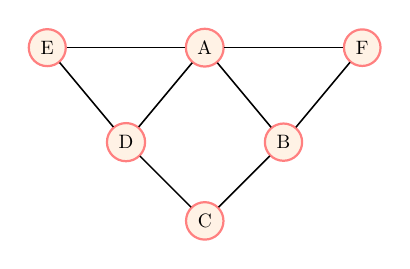
\begin{tikzpicture}
				\node [input_neuron](input0) at (6.5,-0.1)  {D};
				\node [input_neuron] (input1) at (8.5,-0.1)  {B};
				\node [input_neuron] (input2) at (7.5, 1.1) {A};
				\node [input_neuron] (input3) at (7.5, -1.1) {C};
				\node [input_neuron](input4) at (5.5,1.1)  {E};
				\node [input_neuron](input5) at (9.5,1.1)  {F};

				\draw [line width=0.2mm, -] (input0) -- (input2);
				\draw [line width=0.2mm, -] (input0) -- (input3);
				\draw [line width=0.2mm, -] (input1) -- (input2);
				\draw [line width=0.2mm, -] (input1) -- (input3);
				\draw [line width=0.2mm, -] (input0) -- (input4);
				\draw [line width=0.2mm, -] (input2) -- (input4);
				\draw [line width=0.2mm, -] (input1) -- (input5);
				\draw [line width=0.2mm, -] (input2) -- (input5);
			\end{tikzpicture}
			}
			\onslide<3->{\begin{align*}
				&\phi_1(A,E) \phi_2(A,F) \phi_3(B,F) \phi_4(A,B)\\
				&\phi_5(A,D) \phi_6(D,E) \phi_7(B,C) \phi_8(C,D)
			\end{align*}
			}
			\onslide<6->{
			\begin{align*}
				&\phi_1(A,E,D) \phi_2(A,F,B) \phi_3(B,C) \phi_4(C,D)
			\end{align*}
			}
		\end{overlayarea}
		\column{0.5\textwidth}
		\begin{overlayarea}{\textwidth}{\textheight}
			\begin{itemize}\justifying
				\item<1-> Now, what should the factors be?
				\item<2-> We could still have factors which capture pairwise interactions
				\item<4-> But could we do something smarter (and more efficient)
				\item<5-> Instead of having a factor for each pair of nodes why not have it for each maximal clique?
			\end{itemize}
		\end{overlayarea}
	\end{columns}
\end{frame}

\begin{frame}
	\begin{columns}
		\column{0.5\textwidth}
		\begin{overlayarea}{\textwidth}{\textheight}
			\vspace{2cm}
			\centering
			\onslide<2->{
			\tikzstyle{input_neuron}=[circle,draw=red!50,fill=orange!10, thick,scale=0.7]
			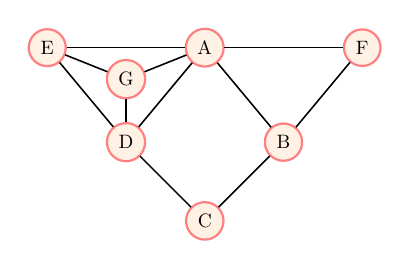
\begin{tikzpicture}
				\node [input_neuron](input0) at (6.5,-0.1)  {D};
				\node [input_neuron] (input1) at (8.5,-0.1)  {B};
				\node [input_neuron] (input2) at (7.5, 1.1) {A};
				\node [input_neuron] (input3) at (7.5, -1.1) {C};
				\node [input_neuron](input5) at (9.5,1.1)  {F};
				\node [input_neuron](input4) at (5.5,1.1)  {E};
				\node [input_neuron](input6) at (6.5,0.7)  {G};
				

				\draw [line width=0.2mm, -] (input0) -- (input2);
				\draw [line width=0.2mm, -] (input0) -- (input3);
				\draw [line width=0.2mm, -] (input1) -- (input2);
				\draw [line width=0.2mm, -] (input1) -- (input3);
				\draw [line width=0.2mm, -] (input0) -- (input4);
				\draw [line width=0.2mm, -] (input2) -- (input4);
				\draw [line width=0.2mm, -] (input1) -- (input5);
				\draw [line width=0.2mm, -] (input2) -- (input5);
				\draw [line width=0.2mm, -] (input0) -- (input6);
				\draw [line width=0.2mm, -] (input2) -- (input6);
				\draw [line width=0.2mm, -] (input4) -- (input6);
			\end{tikzpicture}
			}
		\end{overlayarea}
		\column{0.5\textwidth}
		\begin{overlayarea}{\textwidth}{\textheight}
			\begin{itemize}\justifying
				\item<1-> What if we add one more student?
				\item<3-> What will be the factors in this case?
				\item<4-> Remember, we are interested in maximal cliques
				\item<5-> So instead of having factors $\phi(EAG)$ $\phi(GAD)$ $\phi(EGD)$ we will have a single factor $\phi(AEGD)$ corresponding to the maximal clique
			\end{itemize}
		\end{overlayarea}
	\end{columns}
\end{frame}

\begin{frame}
	\begin{columns}
		\column{0.5\textwidth}
		\begin{overlayarea}{\textwidth}{0.75\textheight}
			\vspace{0.2cm}
			\begin{center}
				\tikzstyle{input_neuron}=[ellipse,draw=red!50,fill=orange!10,thick,scale=0.7]
				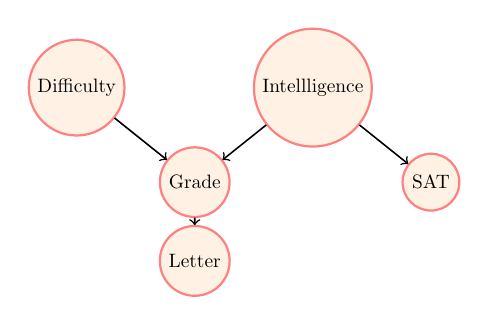
\begin{tikzpicture}
					\node [input_neuron](input0) at (7,-0.1)  {Grade};
					\node [input_neuron] (input1) at (10,-0.1)  {SAT};
					\node [input_neuron] (input2) at (8.5, 1.1) {Intellligence};
					\node [input_neuron] (input3) at (7, -1.1) {Letter};
					\node [input_neuron](input4) at (5.5,1.1)  {Difficulty};

					\draw [line width=0.2mm, ->] (input2) -- (input0);
					\draw [line width=0.2mm, ->] (input0) -- (input3);
					\draw [line width=0.2mm, ->] (input2) -- (input1);
					\draw [line width=0.2mm, ->] (input4) -- (input0);
				\end{tikzpicture}
			\end{center}
			\vspace{-0.4cm}
			\onslide<2->{\footnotesize{
				\begin{itemize}
					\item A distribution P factorizes over a Bayesian Network G if P can be expressed as 
					\begin{align*}
						P(X_1,\ldots,X_n) = \prod_{i=1}^n P(X_i|P_{a_{X_i}})
					\end{align*}
				\end{itemize}
			}}
		\end{overlayarea}
		\column{0.5\textwidth}
		\begin{overlayarea}{\textwidth}{0.75\textheight}
			\onslide<3->{
			\footnotesize{
				\begin{center}
					\tikzstyle{input_neuron}=[circle,draw=red!50,fill=orange!10,thick,scale=0.7]
					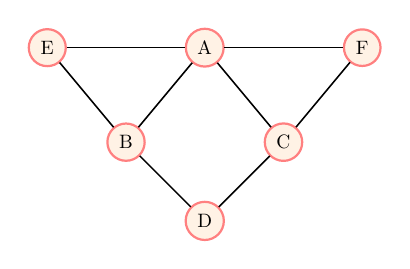
\begin{tikzpicture}
						\node [input_neuron](input0) at (6.5,-0.1)  {B};
						\node [input_neuron] (input1) at (8.5,-0.1)  {C};
						\node [input_neuron] (input2) at (7.5, 1.1) {A};
						\node [input_neuron] (input3) at (7.5, -1.1) {D};
						\node [input_neuron](input4) at (5.5,1.1)  {E};
						\node [input_neuron](input5) at (9.5,1.1)  {F};

						\draw [line width=0.2mm, -] (input0) -- (input2);
						\draw [line width=0.2mm, -] (input0) -- (input3);
						\draw [line width=0.2mm, -] (input1) -- (input2);
						\draw [line width=0.2mm, -] (input1) -- (input3);
						\draw [line width=0.2mm, -] (input0) -- (input4);
						\draw [line width=0.2mm, -] (input2) -- (input4);
						\draw [line width=0.2mm, -] (input1) -- (input5);
						\draw [line width=0.2mm, -] (input2) -- (input5);
					\end{tikzpicture}
				\end{center}
			\vspace{-0.4cm}
			\onslide<4->{\begin{itemize}
				 \item A distribution factorizes over a Markov Network $H$ if P can be expressed as 
				\begin{align*}
					P(X_1,\ldots,X_n) = \frac{1}{Z}\prod_{i=1}^m \phi(D_i)
				\end{align*}
				where each $D_i$ is a complete sub-graph (maximal clique) in $H$
			\end{itemize}}
			}}
		\end{overlayarea}
	\end{columns}
	\onslide<5->{
	\footnotesize{
		\begin{block}{}
		A distribution is a Gibbs distribution parametrized by a set of factors $\Phi = \{ \phi_1(D_1),\ldots,\phi_m(D_m)\}$ if it is defined as
			\vspace{-0.4cm}
			\begin{align*}
				P(X_1, \ldots,X_n) = \frac{1}{Z} \prod_{i=1}^m \phi_i(D_i)
			\end{align*}
			\vspace{-0.3cm}
		\end{block}
	}}
\end{frame}
